%
% eps2pgf_manual.tex
%
% This file is part of Eps2pgf.
%
% Copyright 2008 Paul Wagenaars <paul@wagenaars.org>
%
% Licensed under the Apache License, Version 2.0 (the "License");
% you may not use this file except in compliance with the License.
% You may obtain a copy of the License at
%
%     http://www.apache.org/licenses/LICENSE-2.0
%
% Unless required by applicable law or agreed to in writing, software
% distributed under the License is distributed on an "AS IS" BASIS,
% WITHOUT WARRANTIES OR CONDITIONS OF ANY KIND, either express or implied.
% See the License for the specific language governing permissions and
% limitations under the License.
%

\documentclass{article}

\usepackage{graphicx}
\usepackage{hyperref}
\usepackage{listings}
\lstset{language=[LaTeX]tex, morekeywords={tex,psfrag}, frame=single, basewidth=0.53em}
\usepackage{pgf}

\title{Eps2pgf @VERSION@ User Manual}
\author{Paul Wagenaars}
\date{@BUILDDATE@}

\makeatletter
\hypersetup{
    pdftitle={\@title},
    pdfauthor={\@author}
}
\makeatother

\newcommand{\cmdarg}[2]{
    \par\indent\texttt{#1}
    \smallskip
    \par\indent\indent\parbox{10.9cm}{#2}
    \medskip
}

\begin{document}
    \maketitle
    \tableofcontents

    \section{Introduction}
    Eps2pgf is a PostScript interpreter that converts \href{http://en.wikipedia.org/wiki/Encapsulated_PostScript}{Encapsulated PostScript} (EPS) figures to the \href{http://sourceforge.net/projects/pgf/}{Portable Graphics Format} (PGF). PGF/TikZ is a \TeX{} macro package for generating graphics. It support several back-end drivers, including pdf\TeX{} and Dvips. The major advantage of Eps2pgf is that all texts are typeset by \LaTeX, giving you all the powerful typesetting features and a uniform look of the final document. It has several options to control how text in figures is handled: (i) reproduce text labels accurately (with same font size and formatting as in EPS figure), (ii) copy text labels verbatim (text in EPS figure is \LaTeX{} code), or (iii) replace text labels using \href{http://www.ctan.org/tex-archive/help/Catalogue/entries/psfrag.html}{\textsf{PSfrag}}-compatible rules from a separate file, or using tags embedded in the text labels.

    The goal of Eps2pgf is to support all PostScript figures created by programs regularly used by \LaTeX{} users to create figures, such as MATLAB, Mathematica and Maple. If you encounter a figure that Eps2pgf fails to process, please report it using the bug tracker (\url{http://sourceforge.net/tracker/?group_id=188852&atid=926973}), or send it via email.

    \section{Requirements}
    \begin{itemize}
        \item Java Runtime Environment (version 1.5 or higher)
        \item \LaTeX{}, with the \textsf{pgf} package
    \end{itemize}

    \section{Command line arguments}

    \noindent\texttt{java -jar eps2pgf.jar <\textit{input file}> -o <\textit{output file}>}

    \medskip

    \cmdarg{<\textit{input file}>}{(Encapsulated) PostScript (EPS or PS) input file.}

    \cmdarg{(-o|--output) <\textit{output file}>}{Write output to this file. (default: input file with \texttt{.pgf} extension)}

    \noindent The following arguments are optional:

    \medskip

    \cmdarg{[(-m|--text-mode) <\textit{text mode}>]}{
        Text label handling. Accepted values: \texttt{exact} -- text is reproduced as
        closely as possible, or \texttt{directcopy} -- text is directly copied to the
        output and scanned for embedded \textsf{PSfrag} text replacement rules.
        (default: \texttt{exact})
    }

    \cmdarg{[--text-replace <\textit{text replace file}>]}{File containing \textsf{PSfrag} commands describing text replacements.}

    \cmdarg{[--verbose]}{Display more information during the conversion.}

    \cmdarg{[--version]}{Display version information.}

    \cmdarg{[-h|--help]}{Display program usage.}


    \section{Including PGF figures in \LaTeX{} documents}
    After the the PGF figure has been created it can be included in \LaTeX{} documents. The \textsf{pgf} package is required in order to use PGF figures. A minimal example can be found in figure~\ref{fig:minimal_example}.

    \begin{figure}
        \centering
        \begin{lstlisting}
\documentclass{article}

\usepackage{pgf}

\begin{document}
    \begin{figure}
        \centering
        \input{figure.pgf}
        \caption{pgf figure}
    \end{figure}
\end{document}
        \end{lstlisting}
        \caption{Minimal example of a \LaTeX{} document using a PGF figure.}
        \label{fig:minimal_example}
    \end{figure}


    \section{Text handling}
    Eps2pgf can handle text labels in PostScript figures in various ways. By default it will try to reproduce the text labels as accurately as possible, while using the default font in the \LaTeX{} document. That means that it will use the same font size, style and formatting as in the EPS figure. The center of the text label in the output is aligned with the center of the text label in the PostScript figure.

    In the second mode, invoked using the command line argument \texttt{--text-mode directcopy}, the text in the text labels is directly copied to the PGF figure. This allows you to use custom \LaTeX{} code in the figure. Unless specified otherwise the center of the text label in the output is aligned with the center of the text label in the PostScript figure. Additionally, it is possible to specify anchor, scaling and rotation using the \textsf{PSfrag}-style tag as text label in the PostScript figure:

    \begin{lstlisting}
\tex[pgfanchor][psanchor][scale][rotation]{LaTeX text}
    \end{lstlisting}
    The first four arguments are optional, the last argument is required.
    \begin{itemize}
        \item $[$pgfanchor$]$ --- the \LaTeX{} text reference point. It specifies both the vertical and the horizontal alignment. One of the letters \texttt{t}, \texttt{c}, \texttt{B} or \texttt{b} (top, center, baseline, bottom) specifies the vertical alignment, and one of the letters \texttt{l}, \texttt{c} or \texttt{r} (left, center, right) specifies the horizontal alignment. For example, \verb|[br]| indicates that the anchor is the bottom-right corner of the text label. If the vertical or horizontal alignment is omitted, then \texttt{c} is used. If the argument is omitted completely, \verb|[Bl]| is used.
        \item $[$psanchor$]$ --- the PostScript text reference point. This argument has the same formatting as the pfganchor argument.
        \item $[$scale$]$ --- Scaling factor for font size. It is recommended not to use this parameter, it's better to specify the font size using \LaTeX{}'s font sizing commands. Default: \verb|[1]|.
        \item $[$rotation$]$ --- Extra rotation of the text. The rotation specified here is added to the rotation of the text in the PostScript figure. Default: \verb|[0]|.
        \item $\{$LaTeX text$\}$ --- \LaTeX{} code for the text label.
    \end{itemize}


    It is also possible to use \textsf{PSfrag} text replacement rules, which are specified in a separate file. An external file with replacement rules can be specified using the command line argument \texttt{--text-replace <\textit{text replace file}>}. The rules in this text replacement file specify which text labels must be replace by another text. The file can contain one or more of these rules. These rules follow the exact same syntax as the \textsf{PSfrag} package:
    \begin{lstlisting}
\psfrag{text}[pgfanchor][psanchor][scale][rotation]{LaTeX text}
\psfrag*{text}[pgfanchor][psanchor][scale][rotation]{LaTeX text}
    \end{lstlisting}
    The first and last arguments are required, the other four arguments are optional.
    \begin{itemize}
        \item $\{$text$\}$ --- text in the PostScript figure that will be replaced by the \LaTeX{} text in the last argument.
        \item $[$pgfanchor$]$ --- the \LaTeX{} text reference point. It specifies both the vertical and the horizontal alignment. One of the letters \texttt{t}, \texttt{c}, \texttt{B} or \texttt{b} (top, center, baseline, bottom) specifies the vertical alignment, and one of the letters \texttt{l}, \texttt{c} or \texttt{r} (left, center, right) specifies the horizontal alignment. For example, \verb|[br]| indicates that the anchor is the bottom-right corner of the text label. If the vertical or horizontal alignment is omitted, then \texttt{c} is used. If the argument is omitted completely, \verb|[Bl]| is used.
        \item $[$psanchor$]$ --- the PostScript text reference point. This argument has the same formatting as the pfganchor argument.
        \item $[$scale$]$ --- Scaling factor for font size. It is recommended not to use this parameter, it's better to specify the font size using \LaTeX{}'s font sizing commands. Default: \verb|[1]|.
        \item $[$rotation$]$ --- Extra rotation of the text. The rotation specified here is added to the rotation of the text in the PostScript figure. Default: \verb|[0]|.
        \item $\{$LaTeX text$\}$ --- \LaTeX{} code for the text label.
    \end{itemize}
    Note: Eps2pgf does not correctly handle the starred \verb|\psfrag*| command. Eps2pgf treats the starred version exactly the same as the normal \verb|\psfrag| command, while \textsf{PSfrag} handles it slightly different.

    As a demonstration of the different text modes a figure is converted using different text modes. The original figure, before conversion by Eps2pgf, can be found in figure~\ref{fig:demo_figure_orig}. Converting this figure  with Eps2pgf with default options results in figure~\ref{fig:demo_figure_std}. As you can see it looks pretty similar to the original. It uses the sans-serif font, the label \textsf{\textbf{eq}} is bold, and the font size is the same. The only difference is the font itself.
    Next, the same figure is converted with text mode \texttt{directcopy} and an external file with the following text replacement rules:
    \begin{lstlisting}
\psfrag{xlabel}[cc][cc]{Replaced \texttt{xlabel}}
\psfrag{eq}[bc][tl]{$y = \sin(2x) + \sqrt{x}$}
    \end{lstlisting}
    The resulting figure is figure~\ref{fig:demo_figure_repl}. All labels use the standard text font and formatting. The title label is replaced using the inline \verb|\tex[][]{}| rule. The \textsf{\textbf{eq}} and \textsf{xlabel} labels are replaced using the rules in the external file. Note the usage of the pgf- and psanchor in the rule for the \textsf{\textbf{eq}} label.

    \begin{figure}
        \centering
        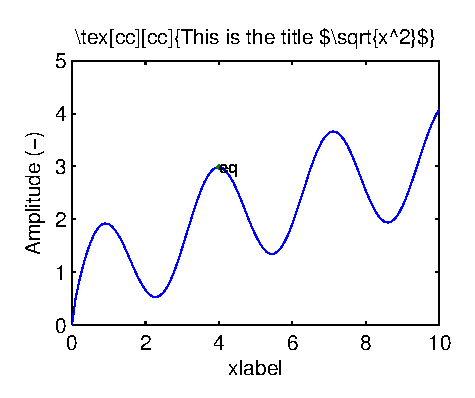
\includegraphics{demo_figure}
        \caption{Original figure create by MATLAB}
        \label{fig:demo_figure_orig}
    \end{figure}

    \begin{figure}
        \centering
        \input{demo_figure_std.pgf}
        \caption{Converted by Eps2pgf with default options}
        \label{fig:demo_figure_std}
    \end{figure}

    \begin{figure}
        \centering
        \input{demo_figure_repl.pgf}
        \caption{Converted by Eps2pgf with text replacements}
        \label{fig:demo_figure_repl}
    \end{figure}

    \section{Copyright and license}
    See the files \texttt{NOTICE.txt} and \texttt{LICENSE.txt}. Or run Eps2pgf with the command line option \texttt{--version}.

\end{document}
